\documentclass[a4paper,12pt]{book}
\usepackage[utf8]{inputenc}
\usepackage[brazil]{babel}
\usepackage{geometry}
\usepackage{setspace}
\usepackage{indentfirst}
\usepackage{hyperref}
\usepackage{graphicx} 
\usepackage{listings}
\usepackage{xcolor}
\usepackage{enumitem}

\setlist[itemize]{itemsep=0pt}

% Configurações da página
\geometry{
	a4paper,
	top=2.5cm,
	bottom=2.5cm,
	left=3cm,
	right=2.5cm
}

% Espaçamento entre linhas
\onehalfspacing

% Recuo da primeira linha dos parágrafos
\setlength{\parindent}{1.25cm}

\hypersetup{
	colorlinks=true,
	linkcolor=blue,
	filecolor=blue,
	urlcolor=blue,
	citecolor=blue,
	anchorcolor=blue,
	breaklinks=true,
	pdftitle={Aprendizagem de Máquina},
	pdfauthor={Giseldo Neo},
	pdfsubject={Assunto do Documento},
	pdfkeywords={aprendizagem de máquina},
	pdfcreator={LaTeX},
	pdfproducer={pdfTeX},
	pdfstartview={FitH},
	pdfpagemode={UseOutlines},
	pdfpagelayout={SinglePage}
}

% Configurações do pacote listings
\lstset{
	basicstyle=\ttfamily\footnotesize,
	keywordstyle=\color{blue},
	commentstyle=\color{green},
	stringstyle=\color{red},
	numbers=left,
	numberstyle=\tiny\color{gray},
	stepnumber=1,
	numbersep=10pt,
	backgroundcolor=\color{white},
	showspaces=false,
	showstringspaces=false,
	showtabs=false,
	frame=single,
	tabsize=2,
	captionpos=b,
	breaklines=true,
	breakatwhitespace=false,
	escapeinside={\%*}{*)}
}

\author{Giseldo Neo}
\title{Aprendizagem de máquina básico}

\begin{document}

\maketitle
\tableofcontents

\chapter{Introdução}

	\section{Inteligência artificial}
		
	O termo ``inteligência'' tem várias definições que dependem do contexto. Isso pode trazer certa confusão no entendimento e delimitação do tema. Menos abrangente, porém mais confuso ainda, é o termo ``inteligência artificial''. Portanto, dado as diversas definições de inteligência artificial (IA), ou \textit{artificial inteligence} em inglês) vamos delimitar um pouco o significado destas palavras.
	
	Nós humanos somos da espécie Homo-Sapiens. Espero que o leitor ainda o seja, pois esse texto pode estar sendo processado para treinar o mais novo modelo de IA como a do filme ``2001 uma odisseia no espaço'', clássico de Kubric, ou como a do mais recente filme ``Ela'', com o ator Joaquim Phenix, espero que com sorte, por um garoto interessado em aprender. 
	
	Homo-Sapiens vem do latim e significa homem sábio \cite{wikipediahumano}. A importância da sapiência (que é um sinônimo de inteligência) é tamanha que define a nossa própria espécie. Porém, dentro do nosso contexto consideramos que um gato e um cachorro são seres dotados de muita inteligência, uma abelha, então nem se fala, praticamente uma cientista. Portanto, seremos mais contidos e reservados quanto ao termo inteligência.
	
	No entanto, várias questões relacionadas a inteligência também guiam inúmeras pesquisas cientificas, por exemplo: como funciona nossa inteligência? Nossa percepção do ambiente é próxima da realidade objetiva? Ainda não é dessa inteligência que estamos falando. Essas perguntas estão mais próxima da neurociência e da filosofia.
	
	Além disso, ``inteligência'' e ``artificial'' são palavras que têm significado implícito para pessoas que não são da área de computação, naturalmente surge o desejo de médicos, advogados, engenheiros (só para citar alguns) de verificar como a “inteligência artificial” pode ser inserida na sua rotina diária. Por exemplo, o meu dentista já quis saber como a IA iria afetar seus procedimentos odontológicos. Porém, ninguém nunca me perguntou em como a ``Transformada de Fourier'' poderia melhorar o seu dia-a-dia, mesmo sabendo que ela já é utilizada em vários domínios do conhecimento e com entusiasmo \cite{wikipediafourier}.
	
	A nossa ``inteligência artificial'' está mais relacionada com a capacidade de realizar coisas que seres inteligentes (um gato, um bebê, ou um cientista) realizam, como por exemplo puxar a mão (ou pata) instantaneamente ao tocar em uma superfície quente (inteligência reativa), ou realizar uma prova de anatomia (inteligência cognitiva). Se conseguimos que programas realizem ações realizadas por entidades dotadas de inteligencia, e realizamos isso  de forma computacional, estamos próximos da nossa definição desejada de ``inteligência artificial''.
	
	Russel e Norvig (2020) em um dos livros mais lidos em todas as universidades do mundo tem uma boa definição sobre esse tema: ``O campo da inteligência artificial [...] tenta não apenas compreender, mas também construir entidades inteligentes'' (tradução nossa) \cite{norvig2002}. Logo, dado o ambicioso desejo de compreender a inteligência, temos o também audacioso objetivo de construir agentes inteligentes dotados dessa inteligência.
	
	A origem do termo ``inteligência artificial'', nesse contexto, é atribuída a John McCarthy, professor de Matemática da Universidade Dartmouth College\cite{blipblog}, ele organizou uma conferência com duração de oito semanas com mais alguns colegas em 1956, alguns anos após a segunda guerra, e desde então o termo vem sendo utilizado para designar parte de conteúdos estudados em ciência da computação. Porém, um pouco antes, o artigo seminal de Alan Turing já demonstrava um bom ensaio sobre as possibilidades de uma máquina inteligente \cite{Turing1950}.
	
	Foi na década de 1970 que o uso da IA começou a ser mais difundido. Esses primeiros sistemas de IA foram chamados de Sistemas Especialistas (veja um exemplo na Figura~\ref{fig:expert})e dependiam muito dos Homo-Sapiens para transformar o conhecimento tácito (baseado em sua experiência) em explicito (formalizado, documentado), que era então codificado na forma de um software contendo regras em lógica formal. O processo de aquisição do conhecimento por esses especialistas acabou sendo um grande obstáculo na adoção em massa dessa abordagem.
	
	\begin{figure}[h]
		\centering
		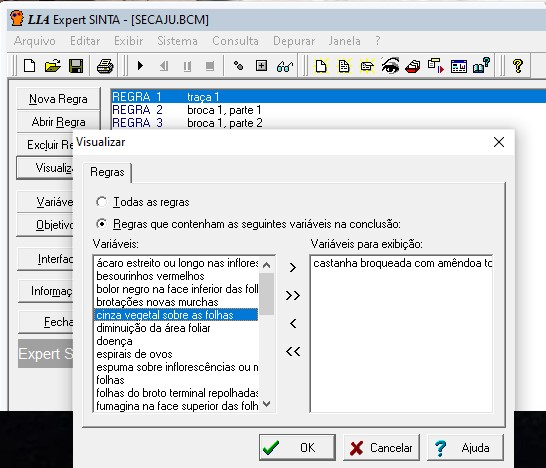
\includegraphics[width=0.7\linewidth]{figuras/expert}
		\caption{ExpertSinta. Uma interface de um Sistema Especialista}
		\label{fig:expert}
	\end{figure}
	
	Nestas últimas décadas houve um crescimento exponencial das tecnologias que  estão ao redor da IA, tais como, o aumento capacidade de processamento e armazenamento dos computadores e a geração de grandes volumes de dados, além dos avanços científicos e tecnológicos em outras áreas, tais como chips supercondutores e eficiência energética.
	
	\section{Aprendizado de Máquina}
	
	O Aprendizado de Máquina (AM) é uma subárea da IA (veja Figura~\ref{fig:iaam}). que foi motivada pelo desenvolvimento de softwares mais independentes da intervenção humana para extração do conhecimento, o que era uma dificuldade nos Sistemas Especialistas. Geralmente aplicações de AM utilizam \textbf{heurísticas} (regra do dedão) que buscam por modelos capazes de representar o conhecimento existente nos dados. 
	
	%% TODO: Definir melhor heurística
	
	\begin{figure}[h]
		\centering
		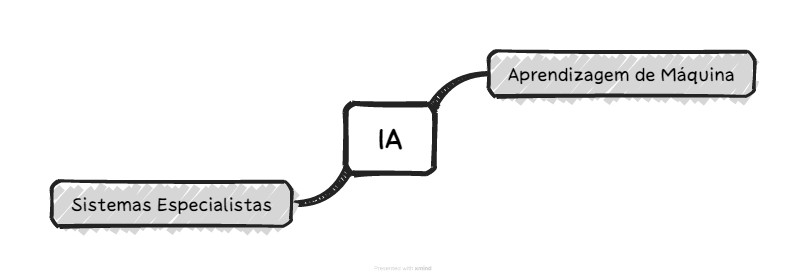
\includegraphics[width=0.9\linewidth]{figuras/ia.png}
		\caption{AM é uma parte da IA}
		\label{fig:iaam}
	\end{figure}
	
	Na Figura~\ref{fig:exemplosam}, é possível identificar alguns usos de AM integrado em diversas atividades cotidianas. São elas, (a) Um smartphone com um assistente de voz fornecendo atualizações meteorológicas. (b) Um sistema de casa inteligente ajustando o termostato com base nas preferências do usuário. (c) Um carro autônomo dirigindo em uma rua movimentada da cidade. (d) Uma plataforma de compras online recomendando produtos a um usuário com base em suas compras anteriores. Essa figura foi criada inclusive com inteligência artificial.
	
	\begin{figure}
		\centering
		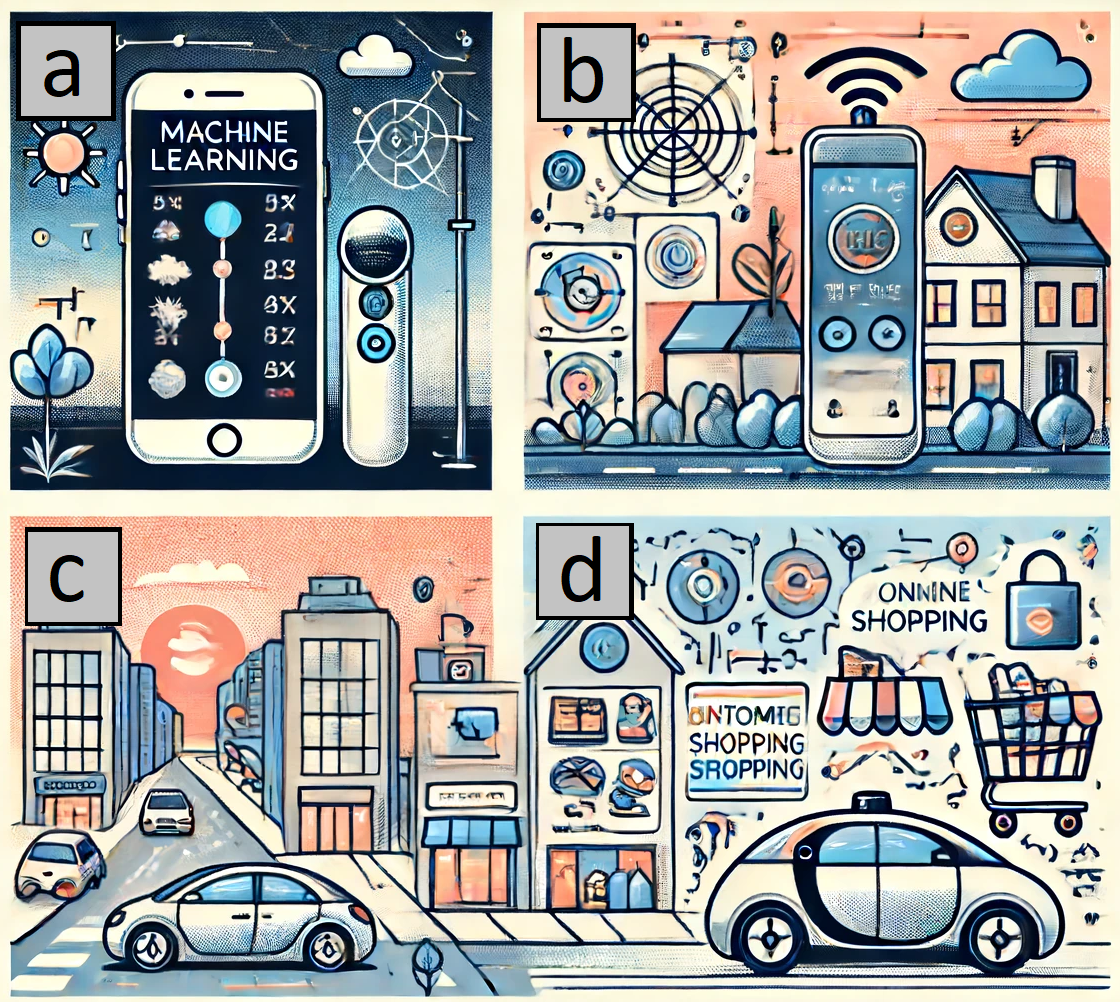
\includegraphics[width=0.7\linewidth]{figuras/exemplos_am}
		\caption{Exemplos AM}
		\label{fig:exemplosam}
	\end{figure}
	 
	\subsection{Classificação}
	
	As tarefas de aprendizado de máquina podem ser divididas entre tarefas preditivas, que visam inferir o atributo alvo de uma nova entrada a partir da exposição prévia aos dados rotulados durante o treinamento do modelo, e descritivas, que buscam extrair padrões dos atributos preditivos. Por conseguinte, uma vez que pertencem a este paradigma, as tarefas de aprendizado descritivas não possuem atributos alvo. Noutras palavras, tarefas preditivas analisarão os atributos preditivos, comparando-os com os atributos alvo (rótulos), ao passo que tarefas descritivas utilizaram os atributos preditivos entre si para buscar por padrões e correlações.
	
	\begin{figure}[h]
		\centering
		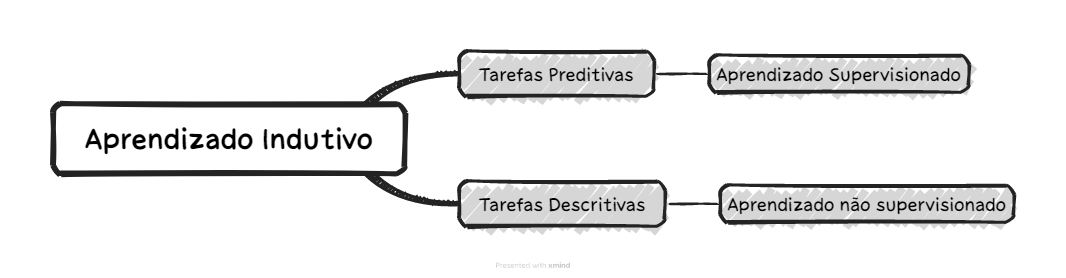
\includegraphics[width=1\linewidth]{figuras/indutivo.png}
		\caption{Classificação AM}
		\label{fig:indutivo}
	\end{figure}
	
	Ambas as tarefas podem ser categorizadas sob o conceito de aprendizado indutivo, que é a capacidade de generalizar a partir de exemplos específicos, isto é, do conjunto de dados de treinamento. Em se tratando de tarefas preditivas, os algoritmos poderão implementar tarefas de classificação, nas quais o atributo alvo (rótulo) é discreto (enumerável ou finito), ou de regressão, em que o atributo alvo (rótulo) é contínuo (não enumerável ou infinito). Já as descritivas distinguem-se entre agrupamento, que busca por similaridades, associação, que busca por padrões frequentes, e sumarização, que resulta em um resumo do conjunto de dados.
	
	% TODO: sinonimo supervisionado e não supervisionado
	
	\subsection{Exemplo de AM}
	
	A seguir um exemplo de modelo preditivo em python. O modelo utiliza o algoritmo SVM e o conjunto de dados iris, que é um conjunto de dados conhecido e bastante utilizado como em demonstrações em outros livros e sites.
	
	\begin{lstlisting}[language=Python, caption={Exemplo de código que usa AM}]
		from sklearn import svm
		from sklearn.datasets import iris
		iris = load_iris()
		X = iris.data
		y = iris.target
		model = svm.SVC()
		model.fit(X, y)
		model.predict([[2., 2., 2., 2.]])
	\end{lstlisting}
	
	%\chapter{Modelo Preditivo}
	
	%\section{Intuição de um modelo preditivo}
	
	%\section{Exemplo de Código}
	
	%Aqui está um exemplo de código em Python:
	
	%\begin{lstlisting}[language=Python, caption={Exemplo de Código Python}]
	%	def hello_world():
	%		print("Hello, world!")
	%	
	%	hello_world()
	%\end{lstlisting}
	
	\chapter{Estatística Básica}
	
	\section{Tipo do Dado}
	
	É necessário classificar o tipo do dado pois os algoritmos de aprendizagem de máquina irão funcionar com determinados tipos. Com o conhecimento do tipo do dado que estamos lidando poderemos realizar as conversões necessárias. 
	
	O tipo do dado pode ser \textbf{numérico} ou \textbf{categórico} (veja a Figura~\ref{fig:tipodado}).
	
	\begin{figure}[!h]
		\centering
		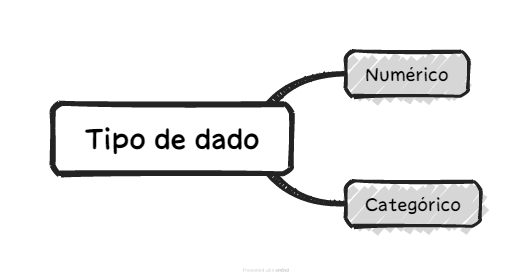
\includegraphics[width=0.7\linewidth]{figuras/tipo_do_dado.png}
		\caption{Tipo de dado}
		\label{fig:tipodado}
	\end{figure}
	
	Dado do tipo \textbf{numérico} é expresso geralmente como um número inteiro ou real. Porém existem casos em que números inteiros expressam dados categóricos. Já o dado do tipo \textbf{categórico} está relacionado a uma classificação do dado. 
	
	\subsection{Dado Numérico}
	
	Já sabemos que um dado do tipo \textbf{numérico} é expresso geralmente como um número inteiro ou real. Além disso, esse tipo de dado ainda pode ser subclassificado em \textbf{contínuo} ou \textbf{discreto} (veja na Figura~\ref{fig:tipodadonumerico}). 
	
	\begin{figure}[!h]
		\centering
		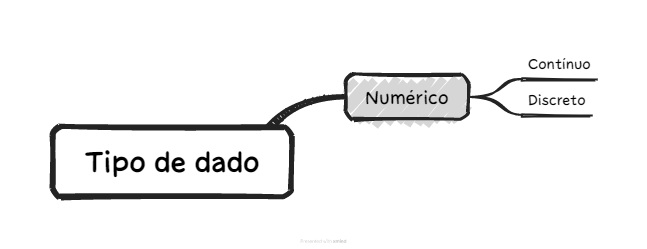
\includegraphics[width=0.8\linewidth]{figuras/tipo_do_dado_numerico.png}
		\caption{Tipo dado numérico}
		\label{fig:tipodadonumerico}
	\end{figure}
	
	Um dado \textbf{numérico contínuo} é quando o dado pode ser qualquer número em um intervalo de numero reais - lembrando que o conjunto de número reais engloba os números inteiros. Geralmente é o resultado de uma medida, por exemplo, a altura dos estudantes é um dado do tipo numérico contínuo.
	
	O dado numérico discreto geralmente é resultado de uma contagem - um número inteiro. Por exemplo, a idade é uma contagem de anos do estudante, logo é um dado do tipo \textbf{numérico discreto}. 
	
	Por exemplo, a idade de um estudante é um dado do tipo \textbf{numérico discreto}. 
	
	Cada linguagem de programação tem tipos de dados específicos para suas variáveis, que estão relacionados as vezes com essa classificação teórica (numérico contínuo ou numerico discreto). Por exemplo no python temos o tipo da variável \textit{int} (inteiro), que é equivalente ao numerico discreto, já o tipo \textit{float} (flutuante) é equivalente ao numérico contínuo.
	
	Aqui está um exemplo de código em Python:
	
	\begin{lstlisting}[language=Python, caption={Exemplo de declaração de variável do tipo inteiro, equivalente ao tipo de dado numérico contínuo.}]
		>>> idade = 25
		>>> type(idade)
		<class 'int'>
	\end{lstlisting}
	
	
	
	
	\subsection{Dado Categórico}
	
	Um dado é do tipo categórico quando ele faz parte de um conjunto, de uma classe ou de uma categoria.
	
	O dado categórico pode ser binário ou ordinal, ou nenhuma das duas subcategorias (Figura~\ref{fig:categoricossubtipos}). 
	
	\begin{figure}
		\centering
		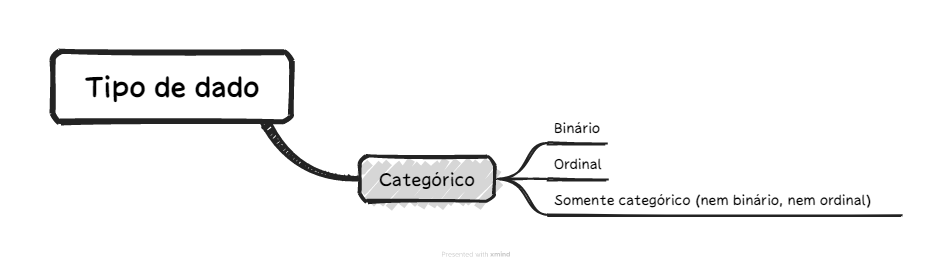
\includegraphics[width=1\linewidth]{figuras/tipo_do_dado_categorico.png}
		\caption{Subtipos Categórico}
		\label{fig:categoricossubtipos}
	\end{figure}
	
	Um exemplo de dado categórico, é uma lista com as cores preferidas dos estudantes, ou o estado civil de uma pessoa.
	
	O dado do tipo categórico binário é um tipo especial quando ele somente pode assumir dois valores no universo de valores possíveis. Por exemplo 0 ou 1, existente ou ausente, true ou false, sim e não.
	
	O dado do tipo categórico ordinal também é um tipo especial, é quando ele faz parte de um conjunto com determinada ordem, por exemplo, imagine a classificação de altura de estudantes somente com os valores alto, médio e baixo. Nesse exemplo existe uma ordem, o aluno com altura classificado como baixo tem uma altura menor do que o aluno com altura média.
	
	
\bibliographystyle{abbrv}
\bibliography{ref}
	
\end{document}